% ATML Programming Assignment 1 -- report.
%
% Official NeurIPS 2026 style (neurips_2026.sty, from the 2026 formatting kit).
% The preprint option shows the author block and drops the review line numbers
% and the "Submitted to NeurIPS" notice. The style fixes the body at 10 pt, the
% "Abstract" heading at 12 pt bold centred, and \footnotesize at no less than
% 8 pt. Use \small (9 pt) for the reference list.

\documentclass{article}

\usepackage[preprint]{neurips_2026}

\usepackage[utf8]{inputenc}
\usepackage[T1]{fontenc}
\usepackage{amsmath,amssymb}
\usepackage{graphicx}
\usepackage{booktabs}
\usepackage{caption}
\usepackage{placeins}
\usepackage{microtype}
\usepackage{url}
\usepackage[colorlinks=true,linkcolor=blue,citecolor=blue,urlcolor=blue]{hyperref}

\graphicspath{{./}}

% Captions at 9 pt (\small); figure and table text stays at or above 8 pt.
\captionsetup{font=small,labelfont=bf,skip=4pt}

\title{Learning Beyond the IID Closed-Set Setting}
\author{Rana Taqveem ul Hassan}

\begin{document}
\maketitle

\begin{abstract}
% Abstract to be written once all four tasks are complete.
Draft compiled with all four tasks.
\end{abstract}

\section{Task 1: Inductive Biases and Feature Representations}

\subsection{Experimental Setup}
% Brief 2-3 sentence overview of dataset (STL-10), architectures (ResNet-50, ViT-B/16,
% CLIP ViT-B/32 with a trained linear head and zero-shot prompts), 500-image balanced
% evaluation subset, and seed 6304.

\subsection{Model's Reliance on Shape, Texture, and Color}

\begin{table}[t]
  \caption{Top-1 accuracy (Acc, \%), change from each method's clean baseline ($\Delta$, pp) and prediction consistency (C, \%) on 500 STL-10 test images (seed 6304). $\dagger$: significant under a paired McNemar test with Holm correction ($p<0.05$). Hue rotation is $30^{\circ}$; patch shuffle uses a $4\times4$ grid.}
  \label{tab:task1_interventions}
  \centering
  \small
  \setlength{\tabcolsep}{4pt}
  \begin{tabular}{lccccccccccc}
    \toprule
    & \textbf{Clean} & \multicolumn{3}{c}{\textbf{Grayscale}} & \multicolumn{3}{c}{\textbf{Hue $30^{\circ}$}} & \multicolumn{3}{c}{\textbf{Patch shuffle}} \\
    \cmidrule(lr){2-2} \cmidrule(lr){3-5} \cmidrule(lr){6-8} \cmidrule(l){9-11}
    \textbf{Method} & Acc & Acc & $\Delta$ & C & Acc & $\Delta$ & C & Acc & $\Delta$ & C \\
    \midrule
    ResNet-50 head       & 97.8 & 96.4 & $-1.4$ & 97.0 & 96.2 & $-1.6$ & 97.0 & 90.0 & $-7.8^{\dagger}$  & 91.8 \\
    ViT-B/16 head        & 98.8 & 96.6 & $-2.2$ & 96.6 & 98.0 & $-0.8$ & 98.4 & 92.6 & $-6.2^{\dagger}$  & 92.8 \\
    CLIP ViT-B/32 head   & 97.8 & 95.4 & $-2.4$ & 95.6 & 97.8 & $+0.0$ & 97.4 & 84.0 & $-13.8^{\dagger}$ & 83.6 \\
    CLIP ViT-B/32 zero-shot & 96.8 & 94.4 & $-2.4^{\dagger}$ & 96.8 & 95.8 & $-1.0$ & 98.4 & 84.0 & $-12.8^{\dagger}$ & 84.4 \\
    \bottomrule
  \end{tabular}
\end{table}

\begin{figure}[t]
  \centering
  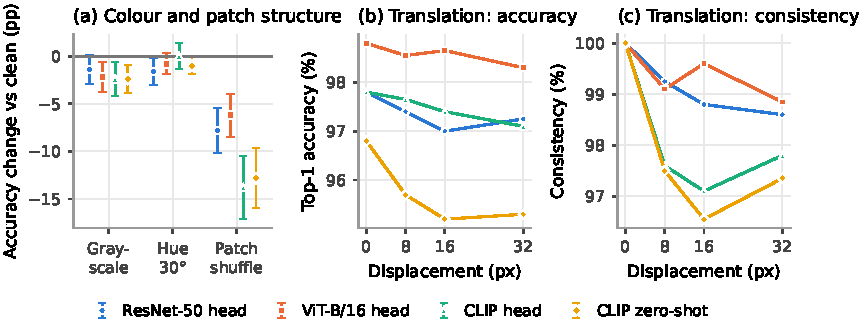
\includegraphics[width=\textwidth]{figures/task1/fig1_interventions.pdf}
  \caption{(a) Accuracy change from the clean baseline with 95\% confidence intervals; intervals crossing zero are within sampling noise. (b) Accuracy and (c) prediction consistency against translation distance, averaged over four directions ($N=500$).}
  \label{fig:task1_interventions}
\end{figure}

Model performance under interventions like color changes (greyscaling or hue modifications) showed no substantial drop in overall performance, suggesting that none of the models gave much importance to the color when making predictions. Removing color altogether cost between 1.4 and 2.4 points, and changing color impacted even less, from 0 to 1.6 points. Although, under the greyscale all four models broke more predictions than they managed to fix, only the zero-shot CLIP change was statistically more reliable.

When the texture of one class is pushed over the shape of another every models showed a strong inclination towards shape bias, with ResNet being the least biased towards shape and appearing to give some importance to texture as well as compared to the rest. Coverage of each model on the cue conflicts gives a different base for these percentages. For ResNet the shape bias is computed from 160 predictions, while for the others from about 180. A lower coverage means the model committed to a cue on fewer images. The models, ViT, the CLIP head, and zero-shot CLIP, predicted a third class on only 17 to 20 of the 200 conflicts, while ResNet did so on 40. Thus, ResNet's shape bias is measured less precisely than the others (Table~\ref{tab:task1_shape_bias}). However it cannot claimed that ResNet's lower coverage follows from its greater reliance on texture or from some other weakness, since a third-class prediction only shows that neither cue won, not which cue caused it.

For the three trained heads (ResNet $+14.5$, CLIP head $+12.0$, ViT $+7.0$ points) the texture class rose into the top two of the ranked class scores more often under conflict than on the clean content image, so texture does influence their scores even though shape still dominates the final decision; zero-shot CLIP showed no such reliable movement.

\begin{table}[t]
  \caption{Cue-conflict decisions on 200 AdaIN conflict images ($\alpha=0.7$). Shape bias $=N_{\text{shape}}/(N_{\text{shape}}+N_{\text{texture}})$; coverage $=(N_{\text{shape}}+N_{\text{texture}})/200$. Brackets: 95\% intervals (bootstrap for shape bias, Wilson for coverage).}
  \label{tab:task1_shape_bias}
  \centering
  \footnotesize
  \setlength{\tabcolsep}{4pt}
  \begin{tabular}{lccccrr}
    \toprule
    \textbf{Method} & \textbf{Shape} & \textbf{Texture} & \textbf{Other} & \textbf{Decisions} & \textbf{Shape bias (\%)} & \textbf{Coverage (\%)} \\
    \midrule
    ResNet-50 head       & 139 & 21 & 40 & 160 & 86.9 [81.4,\,91.9] & 80.0 [73.9,\,85.0] \\
    ViT-B/16 head        & 179 & 4  & 17 & 183 & 97.8 [95.6,\,99.5] & 91.5 [86.8,\,94.6] \\
    CLIP head            & 171 & 11 & 18 & 182 & 94.0 [90.2,\,97.2] & 91.0 [86.2,\,94.2] \\
    CLIP zero-shot       & 172 & 8  & 20 & 180 & 95.6 [92.2,\,98.3] & 90.0 [85.1,\,93.4] \\
    \bottomrule
  \end{tabular}
\end{table}

\begin{figure}[t]
  \centering
  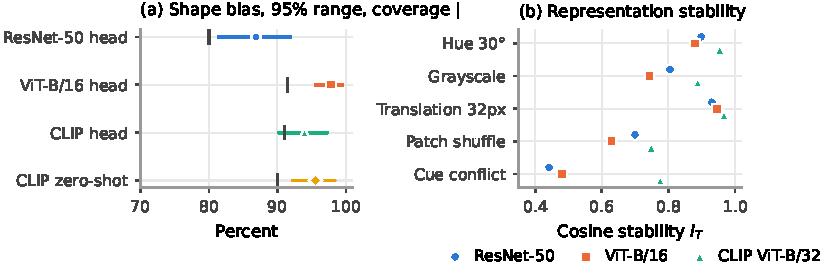
\includegraphics[width=\textwidth]{figures/task1/fig2_cue_and_representation.pdf}
  \caption{(a) Shape bias with 95\% interval, and coverage ($|$), per method. (b) Cosine stability $I_T$ between clean and transformed features per backbone (1 = unchanged); translation averages four 32-pixel shifts. The two CLIP methods share one backbone.}
  \label{fig:task1_cue_representation}
\end{figure}

\begin{figure}[t]
  \centering
  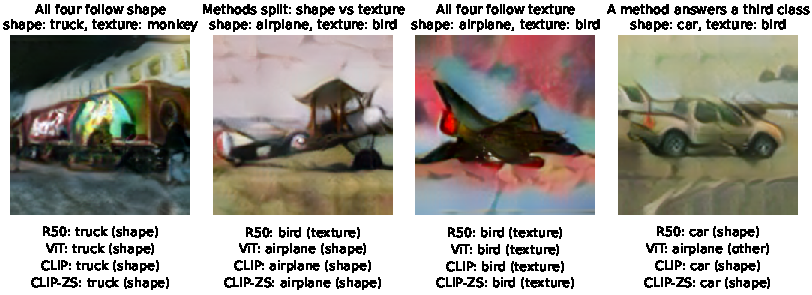
\includegraphics[width=\textwidth]{figures/task1/fig3_cue_examples_compact.pdf}
  \caption{One seeded cue-conflict example per decision pattern (out of 200: all shape 126, split 24, all texture 2, a third class 55), with each method's prediction and whether it follows shape, texture or neither.}
  \label{fig:task1_cue_examples}
\end{figure}

\subsection{Spatial and Positional Invariance}

Models show almost no drop in accuracy and performance with translations. Out of the 48 translation tests (8, 16, and 32 pixels across four directions and four methods), only 8 resulted in 10 or more predictions flipping to negative, with a maximum of 16 (zero-shot CLIP at 16 pixels left), and 7 of these 8 cases belong to zero-shot CLIP. The confidence intervals permit a performance decline of up to approximately 4 points, thus ruling out major degradation from translation while leaving smaller losses possible.

All four drops were statistically reliable, with ResNet and ViT models' performance declining by 6.2 to 7.8 points, where ResNet failed on 39 correct baseline predictions and was unable to correct a single incorrect baseline prediction. The CLIP models appeared to be hit the worst, with the CLIP head breaking 75 predictions while fixing only 6, and overall performance decreasing by 12.8 to 13.8 points. This difference is reliable, as both CLIP methods lost significantly more than ResNet and ViT.

The variation in model performance can be attributed to the changes introduced by each intervention. During the translation interventions, most of the global image and shape structure is preserved. Models still have access to enough global representation, evident from the feature similarity between 0.93 and 0.98 when comparing baseline and translated images, and they therefore retain their accuracy and consistency. This changes substantially with patch shuffling, which moves the patches around and destroys the global spatial arrangement: representational similarity falls to between 0.63 and 0.75, and all models lose accuracy. The correspondence holds when comparing the two interventions, but not when comparing models, since CLIP keeps the highest similarity under shuffling (0.748) while losing the most accuracy ($-13.8$ points), and ViT has the lowest similarity (0.629) with the smallest loss ($-6.2$ points). Furthermore, local features retain significant diagnostic value independently: since patch shuffling keeps every pixel and local texture within each block intact, the models maintain an accuracy of 84.0\% to 92.6\% despite the loss of spatial layout---substantially above chance level. This demonstrates that local texture information sustains the majority of the classification performance, whereas global structure provides the final 6.2 to 13.8 percentage points.

\subsection{Representation Space Analysis}

For all models, feature representation similarity remained quite stable across translations. For color interventions it drops marginally. However, a substantial decline is observed for patch shuffling ViT(0.63) , ResNet(0.70) , CLIP(0.75). Cue conflicts caused the sharpest drop of all, ResNet(0.44), ViT(0.48), but CLIP managed a good performance of 0.78 points.

On translation interventions the features barely moved, (stayed 0.93 $\sim$ 0.98), and accuracy remains stable. The clearest divergence appears with the cue conflicts, where ResNet's representation moves the furthest of all (dropping to 0.442), while its predictions change only slightly, since 139 of 200 still follow the shape class. A possible explanation is that cosine similarity measures how far the representation moved, not what it still contains, so a large movement does not necessarily remove the information the classifier relies on. In these cases, prediction stability and representation stability come apart.

Another interesting finding is observed for ViT on the cue conflicts, where the similarity is 0.505 for stable predictions against 0.264 for flipped ones, showing that the images whose predictions flipped had moved further than those that held. However, under patch shuffling that gap nearly vanishes (0.014 for ResNet), so feature movement barely explains which predictions broke there. Representation change and prediction change therefore agree within a condition, while diverging across conditions.

CLIP lost the most accuracy under shuffling ($-13.8$ points), while ViT moved furthest (0.629 under shuffling) and lost the least ($-6.2$ points).

\begin{figure}[t]
  \centering
  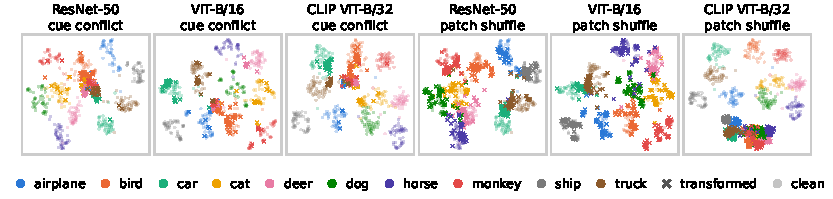
\includegraphics[width=\textwidth]{figures/task1/fig4_tsne_strip.pdf}
  \caption{Joint t-SNE of clean (dots) and transformed (crosses) features per backbone, coloured by class (content class for cue conflicts); coordinates are comparable only within a backbone. In CLIP's patch-shuffle panel the transformed points form a separate cluster although 84.0\% are still classified correctly.}
  \label{fig:task1_tsne}
\end{figure}

CLIP vs CLIP Zero-Shot predicted same class for the same image and they share similar accuracy on the baseline, translations and colour changes. The visible differences come from patch shuffle and cue conflicts. Under patch shuffle the accuracy numbers of the two are identical (84.0\%), yet their agreement on the predicted class drops to 88.2\%, meaning they disagreed on 59 of 500 images, with 22 correct only for the head and 22 correct only for zero-shot. Under cue conflicts agreement is similarly low at 88.0\%, and the texture-rank analysis shows that the transferred texture reliably raised the texture class in the head's top two ($+12.0$ points) but not in zero-shot's ($+0.5$, not reliable). With same backbone embeddings, the two decision rules read those same representations differently, and the trained head is the more texture-sensitive of the two.

\subsection{Architecture and Observation Relationships}

The models differ across their architecture, pretraining data, supervision, and capacity. Such cross-model differences are therefore confounded and cannot be attributed to architecture alone.

Across this experimentation, the one causal claim that can be made about the decision rule comes from comparing CLIP with a trained linear head against zero-shot CLIP. Since both share the same frozen backbone, the same pretraining and identical image embeddings, the observed differences must be driven by the decision rule rather than the representation, as highlighted in their comparison earlier.

A partial architectural link can be drawn between ResNet and ViT. Both were pretrained on the same dataset (ImageNet-1k) with the same supervision (class labels), so data and supervision are held constant. ResNet's reliably lower shape bias (86.9\% vs 97.8\%) and lower coverage (80.0\% vs 91.5\%, driven by 40 third-class predictions concentrated in cases like monkey-to-truck and deer-to-car) indicate a relatively greater reliance on texture than the other three, which is consistent with the convolutional inductive bias reported in the literature. However, the two models also differ in capacity (25M vs 87M parameters) and training recipe (the \texttt{IMAGENET1K\_V2} ResNet weights use heavier augmentation), so architecture cannot be isolated as the cause. The shape bias built into our conflict set raises the absolute level for every method equally, so it explains the high values overall but not the difference between models.

Conversely, CLIP's substantially larger accuracy degradation under patch shuffle ($-12.8$ to $-13.8$ points, compared with $-6.2$ to $-7.8$ for ViT and ResNet) cannot be assigned to architecture, since CLIP differs from ViT in patch size (32 px vs 16 px), supervision (multimodal contrastive) and pretraining scale (400M web pairs) at the same time. The fact that both CLIP variants suffer equally does show that the effect comes from the representation rather than the decision rule.

Definitively isolating these underlying mechanisms would require controlled ablations holding non-architectural factors fixed, such as comparing a supervised ViT-B/16 directly against a CLIP-trained ViT-B/16, or training CNN and Transformer backbones under identical dataset sizes, augmentations, and optimisation recipes.


\FloatBarrier
\section{Task 2: Unsupervised Domain Adaptation}

\subsection{Experimental Setup}
% Brief 2-3 sentence overview: PACS (Photo / Art Painting / Cartoon as labelled sources,
% Sketch as the unlabelled target), ResNet-18 with ImageNet initialisation and a
% seven-class head fine-tuned end to end, frozen BatchNorm running statistics, AdamW at
% lr 1e-4 / weight decay 1e-4, at most 30 epochs with patience 5 on mean source-validation
% macro-F1, domain-balanced batches of 8 per source domain plus 24 target images, seed 6304.

\begin{table}[t]
  \caption{Source-only ERM and three adaptation methods on PACS, Sketch as the unlabelled target. Source columns: macro-F1 on each source validation split (used for checkpoint selection). Sep.: held-out accuracy of a source-vs-target logistic probe (chance 50\%). Lower rows: DANN $\alpha_{\max}$ study (plot in Appendix Fig.~\ref{fig:task2_alignment_study}).}
  \label{tab:task2_methods}
  \centering
  \small
  \setlength{\tabcolsep}{5pt}
  \begin{tabular}{lcccccccc}
    \toprule
    & \multicolumn{4}{c}{\textbf{Source validation (macro-F1)}} & \multicolumn{3}{c}{\textbf{Target: Sketch}} & \\
    \cmidrule(lr){2-5} \cmidrule(lr){6-8}
    \textbf{Method} & Photo & Art & Cartoon & Mean & Acc & Macro-F1 & $\Delta$Acc & \textbf{Sep.} \\
    \midrule
    Source-only ERM         & 95.53 & 92.64 & 95.37 & 94.51 & 55.71 & 55.90 & ---      & 99.86 \\
    DAN (MMD)               & 94.88 & 88.85 & 94.56 & 92.76 & 67.80 & \textbf{66.84} & $+12.09$ & \textbf{89.70} \\
    DANN ($\alpha_{\max}=1$) & 86.73 & 80.30 & 83.25 & 83.43 & 41.51 & 36.71 & $-14.20$ & 100.00 \\
    CDAN                    & 93.87 & 90.26 & 94.12 & 92.75 & 62.36 & 63.12 & $+6.64$  & 98.49 \\
    \midrule
    \multicolumn{9}{l}{\textit{Controlled study: maximum gradient-reversal strength in DANN}} \\
    DANN ($\alpha_{\max}=0.25$) & 96.58 & 91.31 & 94.61 & 94.17 & 28.23 & 20.40 & $-27.49$ & 100.00 \\
    DANN ($\alpha_{\max}=0.5$)  & 94.42 & 87.15 & 91.10 & 90.89 & 38.92 & 32.60 & $-16.80$ & 99.86 \\
    \bottomrule
  \end{tabular}
\end{table}

\subsection{The Source-Only Domain Gap and Its Failure Modes}

\begin{figure}[t]
  \centering
  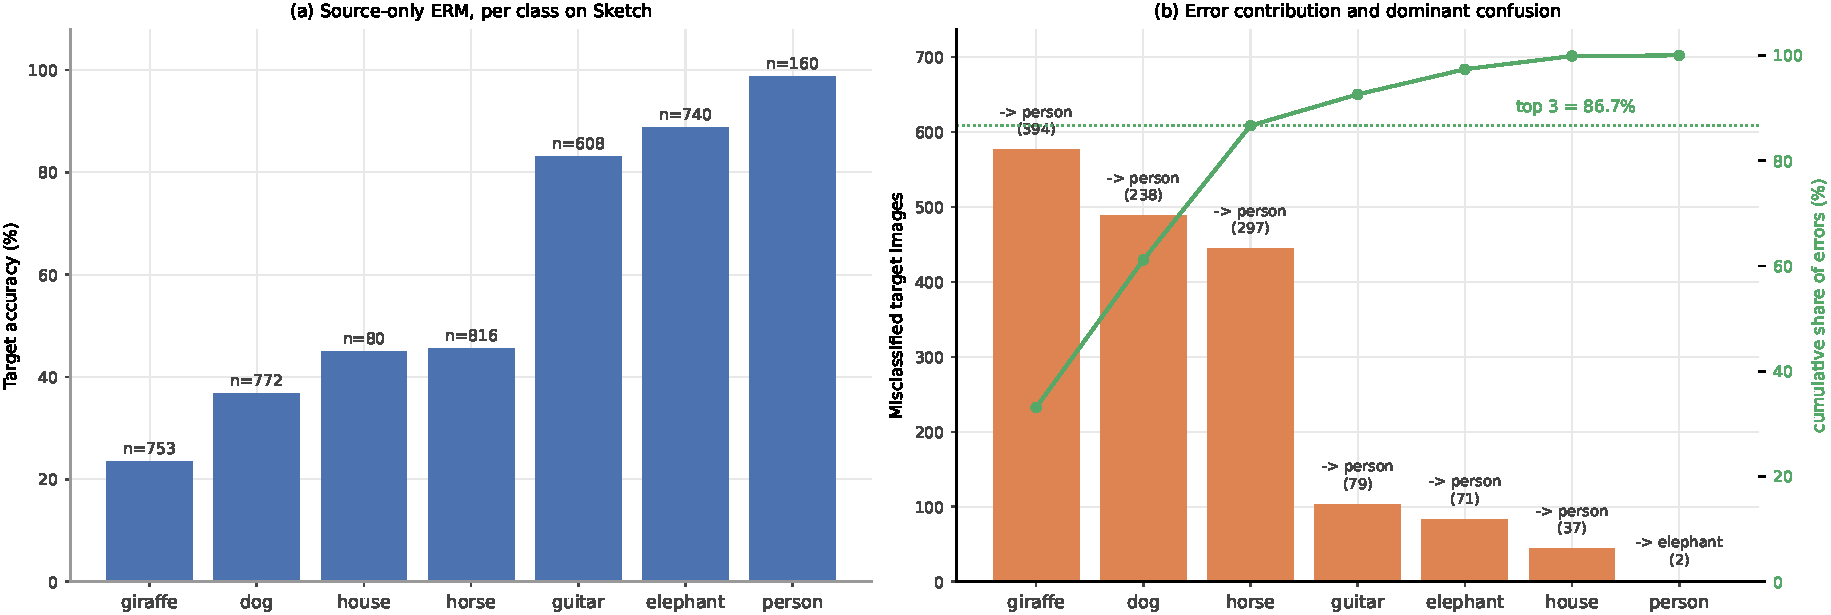
\includegraphics[width=\textwidth]{figures/task2/fig1_erm_failures.pdf}
  \caption{Source-only ERM on Sketch. (a) Per-class accuracy, with target support above each bar. (b) Misclassified images per class with the cumulative error share (right axis), annotated with the class that absorbs most errors.}
  \label{fig:task2_erm_failures}
\end{figure}

The source-only ERM showed a substantial domain gap of 38.61 points (macro-F1) between the source and target domains. Table~\ref{tab:task2_methods} demonstrates that ERM made the model learn class-discriminative source-domain features; however, these features are not directly transferable to the target domain and contain strong domain-specific information, which is clearly visible in the 99.86\% domain-separability score.

The most important target failures were found by accounting for the overall error share of each class: Giraffe, Dog, and Horse accounted for 86.7\% of the overall errors on the target domain. Additionally, the model also displayed a strong bias towards the person class, and the model confused the majority of the classes with person, producing around 1,116 such errors. In contrast, the elephant and guitar classes showed good results, obtaining 88.78\% and 83.06\% accuracy. This shows that the domain shift did not affect each class uniformly.

\subsection{Domain Separability and Target Recognition}

\begin{figure}[t]
  \centering
  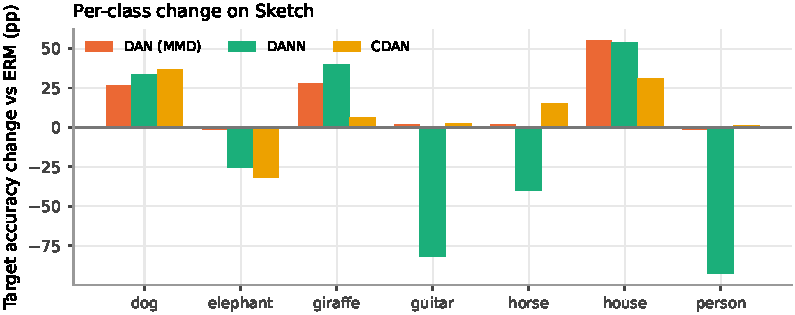
\includegraphics[width=0.75\textwidth]{figures/task2/fig4_per_class.pdf}
  \caption{Per-class change in Sketch accuracy relative to Source-only ERM (pp) for each adaptation method; bars below zero indicate negative transfer. Separability against target macro-F1: Appendix Fig.~\ref{fig:task2_separability}.}
  \label{fig:task2_per_class}
\end{figure}

Across all methods, we see a clear enough pattern: the higher the domain separability between source and target domains, the lower the target accuracy scores. The treatment methods like DAN and CDAN were able to fractionally reduce this separability gap, and as the domain separability scores reduced with these methods, so did the accuracy on the target domain improve. DANN, though it performed miserably because of an unstable optimization flow, shows that it has the highest domain separability score and thus has the lowest target-domain accuracy.

DAN or CDAN, showed better adaptation then others. However, this improvement was not uniform across all of the classes. In DAN, the adaptation improved 5 out of 7 classes, with giraffe improving by 27.89 points, house by 55.00 points, and dog by 26.81 points. However, for elephants and persons, it exhibited negative transfer, declining in performance by 1.62 and 1.25 points. Similarly, CDAN also adapted successfully overall and improved 6 out of 7 classes, except elephant, where its performance decreased by 31.62 points. DANN displayed negative transfer overall and reported terrible performance on guitar, person, horse, and elephant. Its target macro-F1 plummeted by 19.19 points relative to ERM, most likely because of the instability it faced during optimization.

Overall, reduced domain separability can be associated with better performance on target recognition for DAN and CDAN.

\subsection{Class-Conditional versus Marginal Alignment}

The results do not clearly support the claim that class conditioning helps preserve class semantic features better. With DAN, the domain separability score reduced down to 89.69 from 99.86 and showed the best target adaptation performance, reaching 66.84\% macro-F1; however, the individual class-wise macro-F1 for DAN is not uniform across the classes, as it performed really well on 5 out of 7 classes (with giraffe $+27.89$, house $+55.00$, and dog $+26.81$ points), and for elephant and person, it saw a marginal decline.

CDAN also observed an improved domain adaptation and reached a 63.12\% target macro-F1, marginally less than DAN. Overall, it performed well on 6 out of 7 classes and also preserved person and guitar recognition, improving them by 1.25 and 2.47 points, but reduced the adaptation on the elephant class by a massive 31.62 points, and also provided just a 6.51-point gain on the giraffe, whereas on the same giraffe class DAN improved the adaptation by 27.89 points. Thus, the class conditionality might have partially preserved the class-wise consistency, with 6 classes improving; however, it did not manage to improve the overall aggregate for target adaptation.

CDAN does outperform the marginal adversarial alignment DANN, where DANN only reported 36.71\% macro-F1. Overall results may suggest that conditioning can better preserve semantic structure, and it improved aggregate target adaptation relative to ERM but did not outperform DAN,, and stable DAN depicted a good marginal alignment that may outperform CDAN.

\subsection{Effect of Increasing Alignment Strength}

\begin{figure}[t]
  \centering
  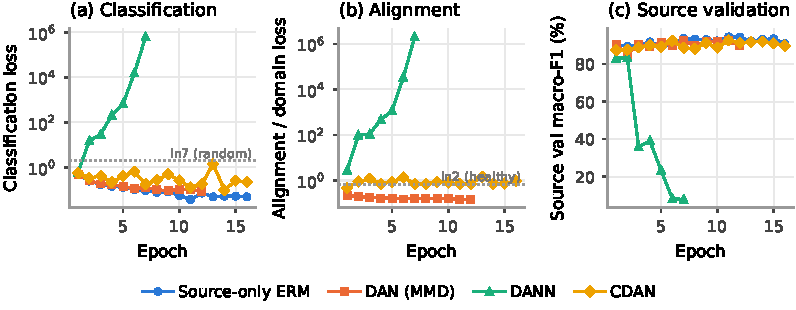
\includegraphics[width=\textwidth]{figures/task2/fig2_training_curves.pdf}
  \caption{(a) Source classification loss; dotted line $\ln 7$ (uniform prediction). (b) Alignment loss: MMD for DAN, domain-classifier loss for DANN and CDAN; dotted line $\ln 2$ (indistinguishable domains). (c) Mean source-validation macro-F1, the selection criterion.}
  \label{fig:task2_training}
\end{figure}

With DANN(1.0) (Figure~\ref{fig:task2_training}) from epoch 2 onwards, the overall optimization became unstable, as the model's classification loss shot up to 15.21 in the second epoch; the training accuracy dropped to 69.80\%, while the validation F1 moved up to 83.43\%, which tells us the model is making some very confident errors as its training accuracy decreases while its validation score remains high. Source-validation performance then collapsed outright from the 3rd epoch, when the validation macro-F1 plummeted from 83.43\% down to 35.96\% and then eventually reached 7.83\%. Both the probabilistic loss and classification performance now show a total failure. The domain accuracy stayed between 42.29\% and 58.18\%; however, the alignment loss increased from 2.78 at the end of the first epoch to 97.49 in the second, reaching 2,013,773.19 in 7 epochs.

As we halve DANN's alignment strength, things do start to get a little better for the source-domain accuracy, as the source macro-F1 gained 7.46 points; however, the reduced alignment strength impacted the target macro-F1, decreasing it by 4.11 points. The pattern repeats when we further reduce the alignment strength, which further increases the model accuracy on source classification; however, it progressively damages target recognition, decreasing target macro-F1 by another 12.19 points. Interestingly, while we have these variations in target F1 score as we decrease the alignment strength, source and target separability remains around 100\%. Therefore, in this scenario, the stronger or weaker adversarial objective failed to produce any measurable domain-invariant features.

In fact, all three DANN configurations remained well below the ERM target macro-F1 of 55.90\%. So, the trade-off between low and high alignment strength had a substantial positive effect on target macro-F1 within the DANN variants; however, stronger alignment destabilized the model's training, and a smaller value further deteriorated the target macro-F1.


\FloatBarrier
\section{Task 3: Domain Generalization}

\subsection{Experimental Setup}
% Brief 2-3 sentence overview: same PACS protocol as Task 2 (Photo / Art Painting / Cartoon
% labelled sources), but Sketch is never loaded until the final evaluation script. ERM is
% the unchanged Task 2 Source-only checkpoint. DAN-DG adds the average pairwise MMD^2 over
% the three source pairs on the 512-d pre-head feature (same three RBF kernels as Task 2,
% lambda_DG = 1); SAM uses non-adaptive SAM with rho = 0.05 on AdamW. Same splits, optimiser,
% epoch budget, patience, 8 images per source domain per batch, and seed 6304; every
% checkpoint selected on mean source-validation macro-F1. Controlled study: lambda_DG in
% {0.1, 1, 10}.

\begin{table}[h]
  \caption{Source validation accuracy / macro-F1 (\%) per domain, with mean and worst, for ERM, DAN-DG and SAM, and the $\lambda_{\mathrm{DG}}$ study below the rule. Checkpoints were selected on mean macro-F1.}
  \label{tab:task3_source}
  \centering
  \small
  \setlength{\tabcolsep}{3pt}
  \begin{tabular}{lccccc}
    \toprule
    \textbf{Method} & Photo & Art & Cartoon & Mean & Worst \\
    \midrule
    ERM                                & 96.11 / 95.53 & 92.68 / 92.64 & 94.67 / 95.37 & 94.49 / 94.51 & 92.68 / 92.64 \\
    DAN-DG ($\lambda_{\mathrm{DG}}=1$) & 94.31 / 93.24 & 89.02 / 89.35 & 92.11 / 92.09 & 91.82 / 91.56 & 89.02 / 89.35 \\
    SAM ($\rho=0.05$)                  & 97.31 / 96.77 & 92.44 / 92.34 & 95.74 / 96.23 & 95.16 / 95.12 & 92.44 / 92.34 \\
    \midrule
    \multicolumn{6}{l}{\textit{Controlled study: alignment strength $\lambda_{\mathrm{DG}}$ in DAN-DG}} \\
    DAN-DG ($\lambda_{\mathrm{DG}}=0.1$) & 95.51 / 94.67 & 91.46 / 91.24 & 91.68 / 92.17 & 92.89 / 92.69 & 91.46 / 91.24 \\
    DAN-DG ($\lambda_{\mathrm{DG}}=10$)  & 41.32 / 21.54 & 25.12 / 15.39 & 18.12 / 11.24 & 28.19 / 16.06 & 18.12 / 11.24 \\
    \bottomrule
  \end{tabular}
\end{table}

\begin{table}[h]
  \caption{Sketch accuracy and macro-F1, change against ERM (pp), source-domain separability (3-way probe, chance 33.3\%) and the sharpness proxy: validation loss $\mathcal L$, loss after a radius-0.05 ascent step $\mathcal L_{+\epsilon}$, and their difference $\Delta_{\mathrm{sharp}}$ (96 images). Plots: Appendix Figs.~\ref{fig:task3_alignment} and \ref{fig:task3_diagnostics}.}
  \label{tab:task3_target}
  \centering
  \small
  \setlength{\tabcolsep}{4pt}
  \begin{tabular}{lcccccccc}
    \toprule
    & \multicolumn{4}{c}{\textbf{Sketch}} & & \multicolumn{3}{c}{\textbf{Sharpness proxy}} \\
    \cmidrule(lr){2-5} \cmidrule(lr){7-9}
    \textbf{Method} & Acc & Macro-F1 & $\Delta$Acc & $\Delta$F1 & \textbf{Sep.} & $\mathcal L$ & $\mathcal L_{+\epsilon}$ & $\Delta_{\mathrm{sharp}}$ \\
    \midrule
    ERM                                & 55.71 & 55.90 & ---       & ---       & 86.38 & 0.192 & 0.792 & 0.600 \\
    DAN-DG ($\lambda_{\mathrm{DG}}=1$) & 68.44 & 72.37 & $+12.73$  & $+16.46$  & 80.07 & 0.217 & 0.849 & 0.631 \\
    SAM ($\rho=0.05$)                  & 64.55 & 67.64 & $+8.83$   & $+11.74$  & 86.38 & 0.073 & 0.214 & 0.141 \\
    \midrule
    \multicolumn{9}{l}{\textit{Controlled study: alignment strength $\lambda_{\mathrm{DG}}$ in DAN-DG}} \\
    DAN-DG ($\lambda_{\mathrm{DG}}=0.1$) & 71.70 & 72.63 & $+15.98$ & $+16.73$ & 81.40 & 0.150 & 0.887 & 0.737 \\
    DAN-DG ($\lambda_{\mathrm{DG}}=10$)  & 10.56 & 7.84  & $-45.15$ & $-48.06$ & 48.84 & 1.855 & 4.103 & 2.248 \\
    \bottomrule
  \end{tabular}
\end{table}

\subsection{Source Validation as a Predictor of Sketch Performance}



\begin{table}[t]
  \caption{Per-class Sketch accuracy (\%) with the change against ERM (pp) in brackets, including target-aware DAN from Task 2. Plots: Appendix Figs.~\ref{fig:task3_alignment} and \ref{fig:task3_vs_task2}.}
  \label{tab:task3_per_class}
  \centering
  \small
  \setlength{\tabcolsep}{2.5pt}
  \begin{tabular}{lcccccc}
    \toprule
    & & & \multicolumn{3}{c}{\textbf{Task 3}} & \textbf{Task 2} \\
    \cmidrule(lr){4-6} \cmidrule(lr){7-7}
    \textbf{Class} & Support & ERM & DAN-DG ($\lambda{=}1$) & SAM & DAN-DG ($\lambda{=}10$) & DAN \\
    \midrule
    \texttt{dog} & 772 & 36.79 & 36.66 ($-0.13$) & 30.18 ($-6.61$) & 11.79 ($-25.00$) & 63.60 ($+26.81$) \\
    \texttt{elephant} & 740 & 88.78 & 96.22 ($+7.43$) & 98.51 ($+9.73$) & 30.41 ($-58.38$) & 87.16 ($-1.62$) \\
    \texttt{giraffe} & 753 & 23.51 & 44.89 ($+21.38$) & 56.31 ($+32.80$) & 0.00 ($-23.51$) & 51.39 ($+27.89$) \\
    \texttt{guitar} & 608 & 83.06 & 95.56 ($+12.50$) & 85.36 ($+2.30$) & 0.66 ($-82.40$) & 84.87 ($+1.81$) \\
    \texttt{horse} & 816 & 45.59 & 73.04 ($+27.45$) & 55.64 ($+10.05$) & 0.00 ($-45.59$) & 47.67 ($+2.08$) \\
    \texttt{house} & 80 & 45.00 & 93.75 ($+48.75$) & 81.25 ($+36.25$) & 63.75 ($+18.75$) & 100.00 ($+55.00$) \\
    \texttt{person} & 160 & 98.75 & 65.00 ($-33.75$) & 70.00 ($-28.75$) & 27.50 ($-71.25$) & 97.50 ($-1.25$) \\
    \bottomrule
  \end{tabular}
\end{table}

Good performance on the source domain does not guarantee good performance on the target domain, and this is visible via the results (Tables~\ref{tab:task3_source} and~\ref{tab:task3_target}). Their worst-performing source macro-F1 is 89.35 and 92.34, respectively. While establishing a possible link between the validation numbers of source domains and the test numbers of the target domains, ERM, as anticipated, performed worst in the target domain, whereas DAN-DG has the lowest mean source accuracy of 91.82 and best target accuracy/macro-F1 of 68.44/72.37. SAM has performed the highest mean source accuracy of 95.16, but still its target accuracy is 3.89 points lower than DAN-DG. Therefore, it is difficult to establish that source validation performance reliably predicts performance on Sketch.

ERM performs very poorly on Sketch for giraffe, dog, horse, and house, with accuracies of 23.51\%, 36.79\%, 45.59\%, and 45.00\%, whereas in the case of DAN-DG, 5 out of 7 classes gained points (house by 48.75 points, horse by 27.45, giraffe by 21.38, and guitar by 12.50). However, for the person, the performance declined by 33.75 points. Therefore, high aggregate source performance hides substantial target-specific class failures, particularly the degradation of person and the continued difficulty of dog recognition.

The art domain is recorded as the worst across all three methods.

\FloatBarrier
\subsection{Source-Domain Invariance and Class-Discriminative Information}

\begin{figure}[t]
  \centering
  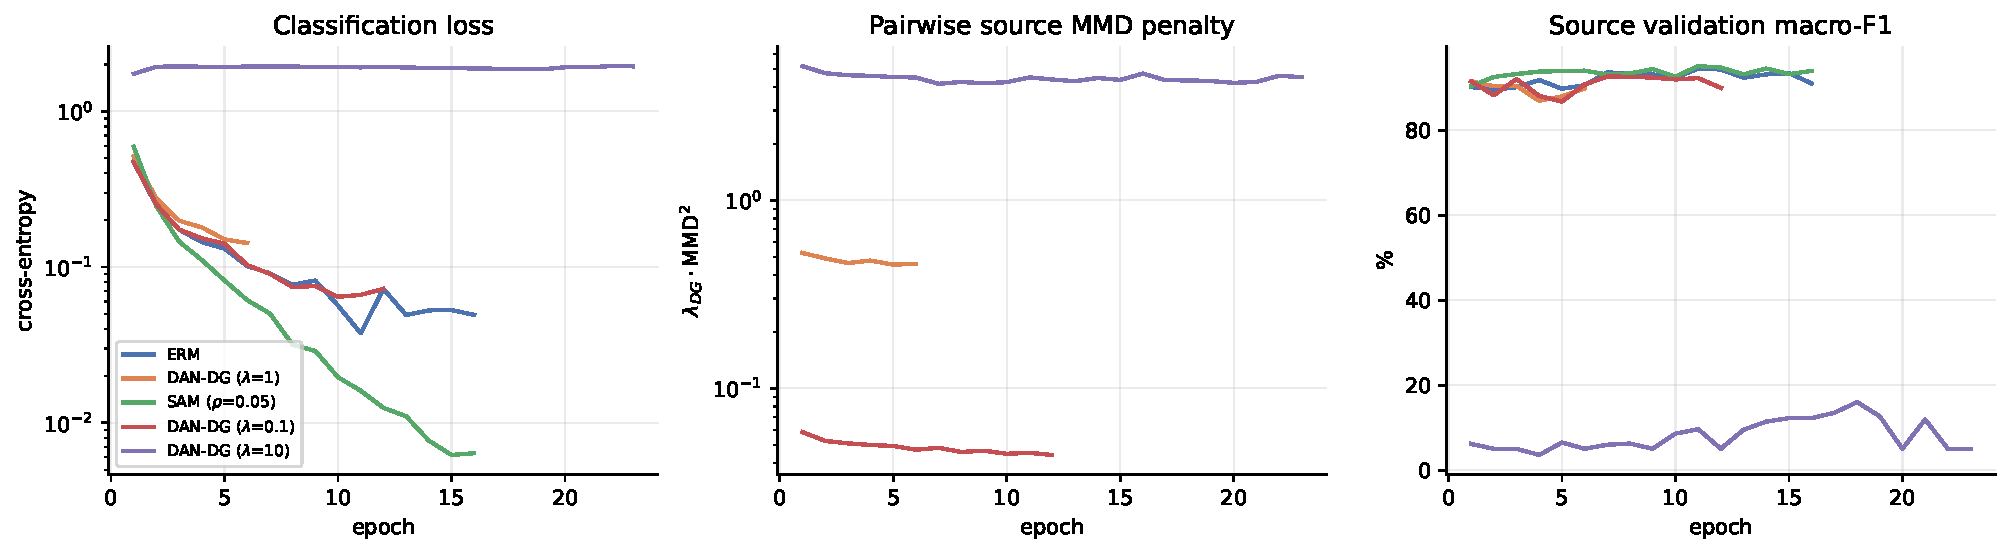
\includegraphics[width=\textwidth]{figures/task3/fig1_training_curves.pdf}
  \caption{(a) Classification loss, (b) weighted pairwise source MMD penalty for DAN-DG, (c) mean source-validation macro-F1. ERM is the reused Task 2 run; curves end at early stopping.}
  \label{fig:task3_training}
\end{figure}



DAN-DG made the observed source domains slightly less distinguishable, as shown by the source-domain separability score, which decreases to 80.07\% compared with 86.38\% under ERM. Its performance on Sketch also got better, and it reported an increase in macro-F1 from 55.90 to 72.37. These numbers appear to support the claim; however, the results change drastically when $\lambda_{\mathrm{DG}}$ is increased to 10. The separability score fell to 48.84\%, but the macro-F1 on both the Sketch and the source just collapsed to 7.84\% and 16.06\%, respectively. Class-wise, 6 out of 7 classes lost substantial points: guitar fell by 82.40 points, person by 71.25, elephant by 58.38, and both giraffe and horse reached 0\% accuracy. Moreover, in the case of SAM and ERM, the separability is identical at 86.38\%, yet SAM's Sketch macro-F1 is 67.64 against ERM's 55.90. This suggests that excessive source alignment does remove domain-discriminative features, making domains more difficult to distinguish; however, at the same time, it destroys the core semantic structure required for classification. Therefore, moderate invariance among the domains partially improves Sketch recognition, while a stronger push results in loss of critical class-discriminative information, resulting in poor performance on the target domain.

\FloatBarrier
\subsection{Local Stability and Sketch Performance}



A lower common sharpness proxy under given perturbation partially supports the claim about local stability, but it does not establish that the overall loss surface is flatter and will generalize better on any domain shifts. With SAM perturbation the loss increased by just 0.141, as compared to ERM and DAN-DG, which reported a change of 0.600 and 0.631, respectively. Therefore, the local stability ranking is
\[ \text{SAM} < \text{ERM} < \text{DAN-DG}. \]
However, it does not establish that the local stability ranking enables better performance on the target domain, because on the target domain the performance of each model is
\[ \text{DAN-DG} > \text{SAM} > \text{ERM}. \]
DAN-DG reported the highest sensitivity to a minor perturbation; however, its Sketch macro-F1 is the highest (72.37\%), whereas SAM is much flatter as per the proxy ranking, but it reaches 67.64\%. Nevertheless, SAM does improve over ERM by 8.83 accuracy points and 11.74 macro-F1 points, suggesting that local parameter stability may contribute to some extent to better generalization, but it is difficult to confirm that in every setting SAM will result in better performance on target domains.

\FloatBarrier
\subsection{Target-Aware DAN versus Target-Free DAN-DG}

Both methods improve substantially over the shared ERM baseline (Table~\ref{tab:task3_target_access})

\begin{table}[h]
  \caption{Target-aware DAN (Task 2) and target-free DAN-DG (Task 3) against the shared ERM checkpoint.}
  \label{tab:task3_target_access}
  \centering
  \small
  \begin{tabular}{llcc}
    \toprule
    \textbf{Method} & \textbf{Training alignment} & \textbf{Sketch accuracy} & \textbf{Sketch F1} \\
    \midrule
    ERM           & None                            & 55.71\% & 55.90\% \\
    Task 2 DAN    & Source versus unlabeled Sketch  & 67.80\% & 66.84\% \\
    Task 3 DAN-DG & Pairwise observed sources only  & 68.44\% & 72.37\% \\
    \bottomrule
  \end{tabular}
\end{table}

DAN used unlabeled Sketch data to align the source features and improved over ERM by 12.09 accuracy points and 10.93 macro-F1 points. DAN-DG, which never had access to the target data (sketches) during training, improved by 12.73 accuracy points and 16.46 macro-F1 points. DAN-DG exceeds target-aware DAN by 0.64 accuracy points and 5.53 macro-F1 points.

This suggests that access to unlabeled Sketch data did not provide a substantial empirical advantage. Instead, it highlights that DAN-DG was able to learn the cross-domain invariances, which resulted in source-target alignment. However, this does not establish that unlabeled Sketch data has no value, and several limitations prevent this from being a complete causal attribution.



The whole experiment is limited to a single seed, 6304, a different seed might have produced different results.

DAN and DAN-DG work on different distributions; the DAN objective aligns source and target domain features given by  \(\mathcal L_{\mathrm{align}}^{\mathrm{DAN}} = \operatorname{MMD}^2 \left( F(X_P\cup X_A\cup X_C), F(X_S) \right).\) whereas DAN-DG tries to learn invariances among the source domains:
\[ \mathcal L_{\mathrm{align}}^{\mathrm{DAN-DG}} = \frac{ \operatorname{MMD}^2(P,A) + \operatorname{MMD}^2(P,C) + \operatorname{MMD}^2(A,C) }{3}. \]
In DAN, the pooled comparison between the source and target can hide the differences between the individual source domains; however, the pairwise terms in DAN-DG ensure that these differences are accounted for.


\FloatBarrier
\section{Task 4: Open-Set Recognition}

\subsection{Experimental Setup}
% Brief 2-3 sentence overview: CIFAR-10 as the ten known classes; CIFAR-100 used only at
% final evaluation, 100 images per unknown class. Near unknowns: bus, pickup truck,
% motorcycle, tractor, wolf, fox, leopard, camel (800 images). Far unknowns: bottle, bowl,
% chair, clock, keyboard, mushroom, sunflower, wardrobe (800 images). CIFAR ResNet-18
% (3x3 stride-1 first conv, no max-pool, 32x32 input), SGD lr 0.1 / momentum 0.9 / weight
% decay 5e-4 with cosine decay, batch 128, 100 epochs, seed 6304, checkpoint = best CIFAR-10
% validation accuracy. GCSC = same recipe + RandAugment(2 ops, magnitude 9). PROSER =
% fine-tuned from the Vanilla checkpoint for 50 epochs with 5 dummy classifiers and
% layer-2 manifold mixup (Beta(2,2)). Rejection threshold = 95th percentile of
% unknownness on CIFAR-10 validation, so about 95% of known examples are accepted.

\subsection{Semantic Similarity and Rejection}

\begin{table}[h]
  \caption{Post-hoc scores on the frozen Vanilla model: AUROC (CIFAR-10 test against each unknown group) and rejection at the threshold that accepts 95\% of CIFAR-10 validation images. Known: CIFAR-10 test images accepted. 800 images per unknown group.}
  \label{tab:task4_posthoc}
  \centering
  \small
  \setlength{\tabcolsep}{4pt}
  \begin{tabular}{lccccccc}
    \toprule
    & \multicolumn{3}{c}{\textbf{AUROC}} & & \multicolumn{3}{c}{\textbf{Rejection (\%)}} \\
    \cmidrule(lr){2-4} \cmidrule(lr){6-8}
    \textbf{Score} & Near & Far & All & Known (\%) & Near & Far & All \\
    \midrule
    MSP         & \textbf{0.814} & 0.887 & 0.850 & 94.09 & 31.38 & 46.38 & 38.88 \\
    MLS         & 0.802 & 0.883 & 0.842 & 94.22 & \textbf{34.75} & \textbf{54.13} & \textbf{44.44} \\
    Energy      & 0.802 & 0.883 & 0.843 & 94.41 & 34.50 & 53.25 & 43.88 \\
    Mahalanobis & 0.795 & \textbf{0.911} & \textbf{0.853} & 94.36 & 27.75 & 51.38 & 39.56 \\
    \bottomrule
  \end{tabular}
\end{table}



\begin{table}[h]
  \caption{Most confidently accepted near and far unknowns (Vanilla, MLS); an image is accepted when its score is below the threshold $-6.058$. Per-class acceptance: Appendix Fig.~\ref{fig:task4_unknown_classes}.}
  \label{tab:task4_failures}
  \centering
  \small
  \begin{tabular}{llcc@{\hspace{18pt}}llc}
    \toprule
    \multicolumn{3}{c}{\textbf{Near unknowns}} & & \multicolumn{3}{c}{\textbf{Far unknowns}} \\
    \cmidrule(lr){1-3} \cmidrule(lr){5-7}
    Unknown & Predicted & Score & & Unknown & Predicted & Score \\
    \midrule
    wolf          & dog        & $-12.12$ & & keyboard  & bird     & $-12.15$ \\
    fox           & cat        & $-12.04$ & & mushroom  & bird     & $-11.89$ \\
    bus           & truck      & $-11.60$ & & chair     & airplane & $-11.77$ \\
    tractor       & ship       & $-11.54$ & & keyboard  & truck    & $-11.54$ \\
    pickup truck  & automobile & $-11.46$ & & sunflower & bird     & $-11.52$ \\
    \bottomrule
  \end{tabular}
\end{table}

The semantic similarity of certain classes made the rejection substantially harder for the model. With the vanilla MLS measure of unknownness, the model rejected only \(34.75\%\) near unknowns with an AUROC of \(0.802\), whereas it rejected around \(54.13\%\) far unknowns with an AUROC of \(0.883\).

The most frequently accepted unknown classes were among pickup trucks (\(91\%\) accepted, most often as automobiles), bus (\(82\%\), most often as truck), and wolf (\(77\%\), most often as dog). Similarly, the model confused wolves as dogs and leopards as cats, indicating that the visual and semantic similarity among some of the unknown categories with known ones is quite plausible, making rejection difficult for the model.

Among some of the semantically far unknowns, the wardrobe (\(68\%\)), bowl (\(53\%\)), and sunflower (\(47\%\)) had the highest acceptance rates. Additional confident failures are the keyboard/mushroom by bird and chair by airplane. The high acceptance rates for these failed semantically far unknowns suggest that the classifier might have responded to incidental similarities in shape, color or some other spurious correlations like background rather than some discriminative class features.

\FloatBarrier
\subsection{What the Novelty Scores Capture}

\begin{figure}[t]
  \centering
  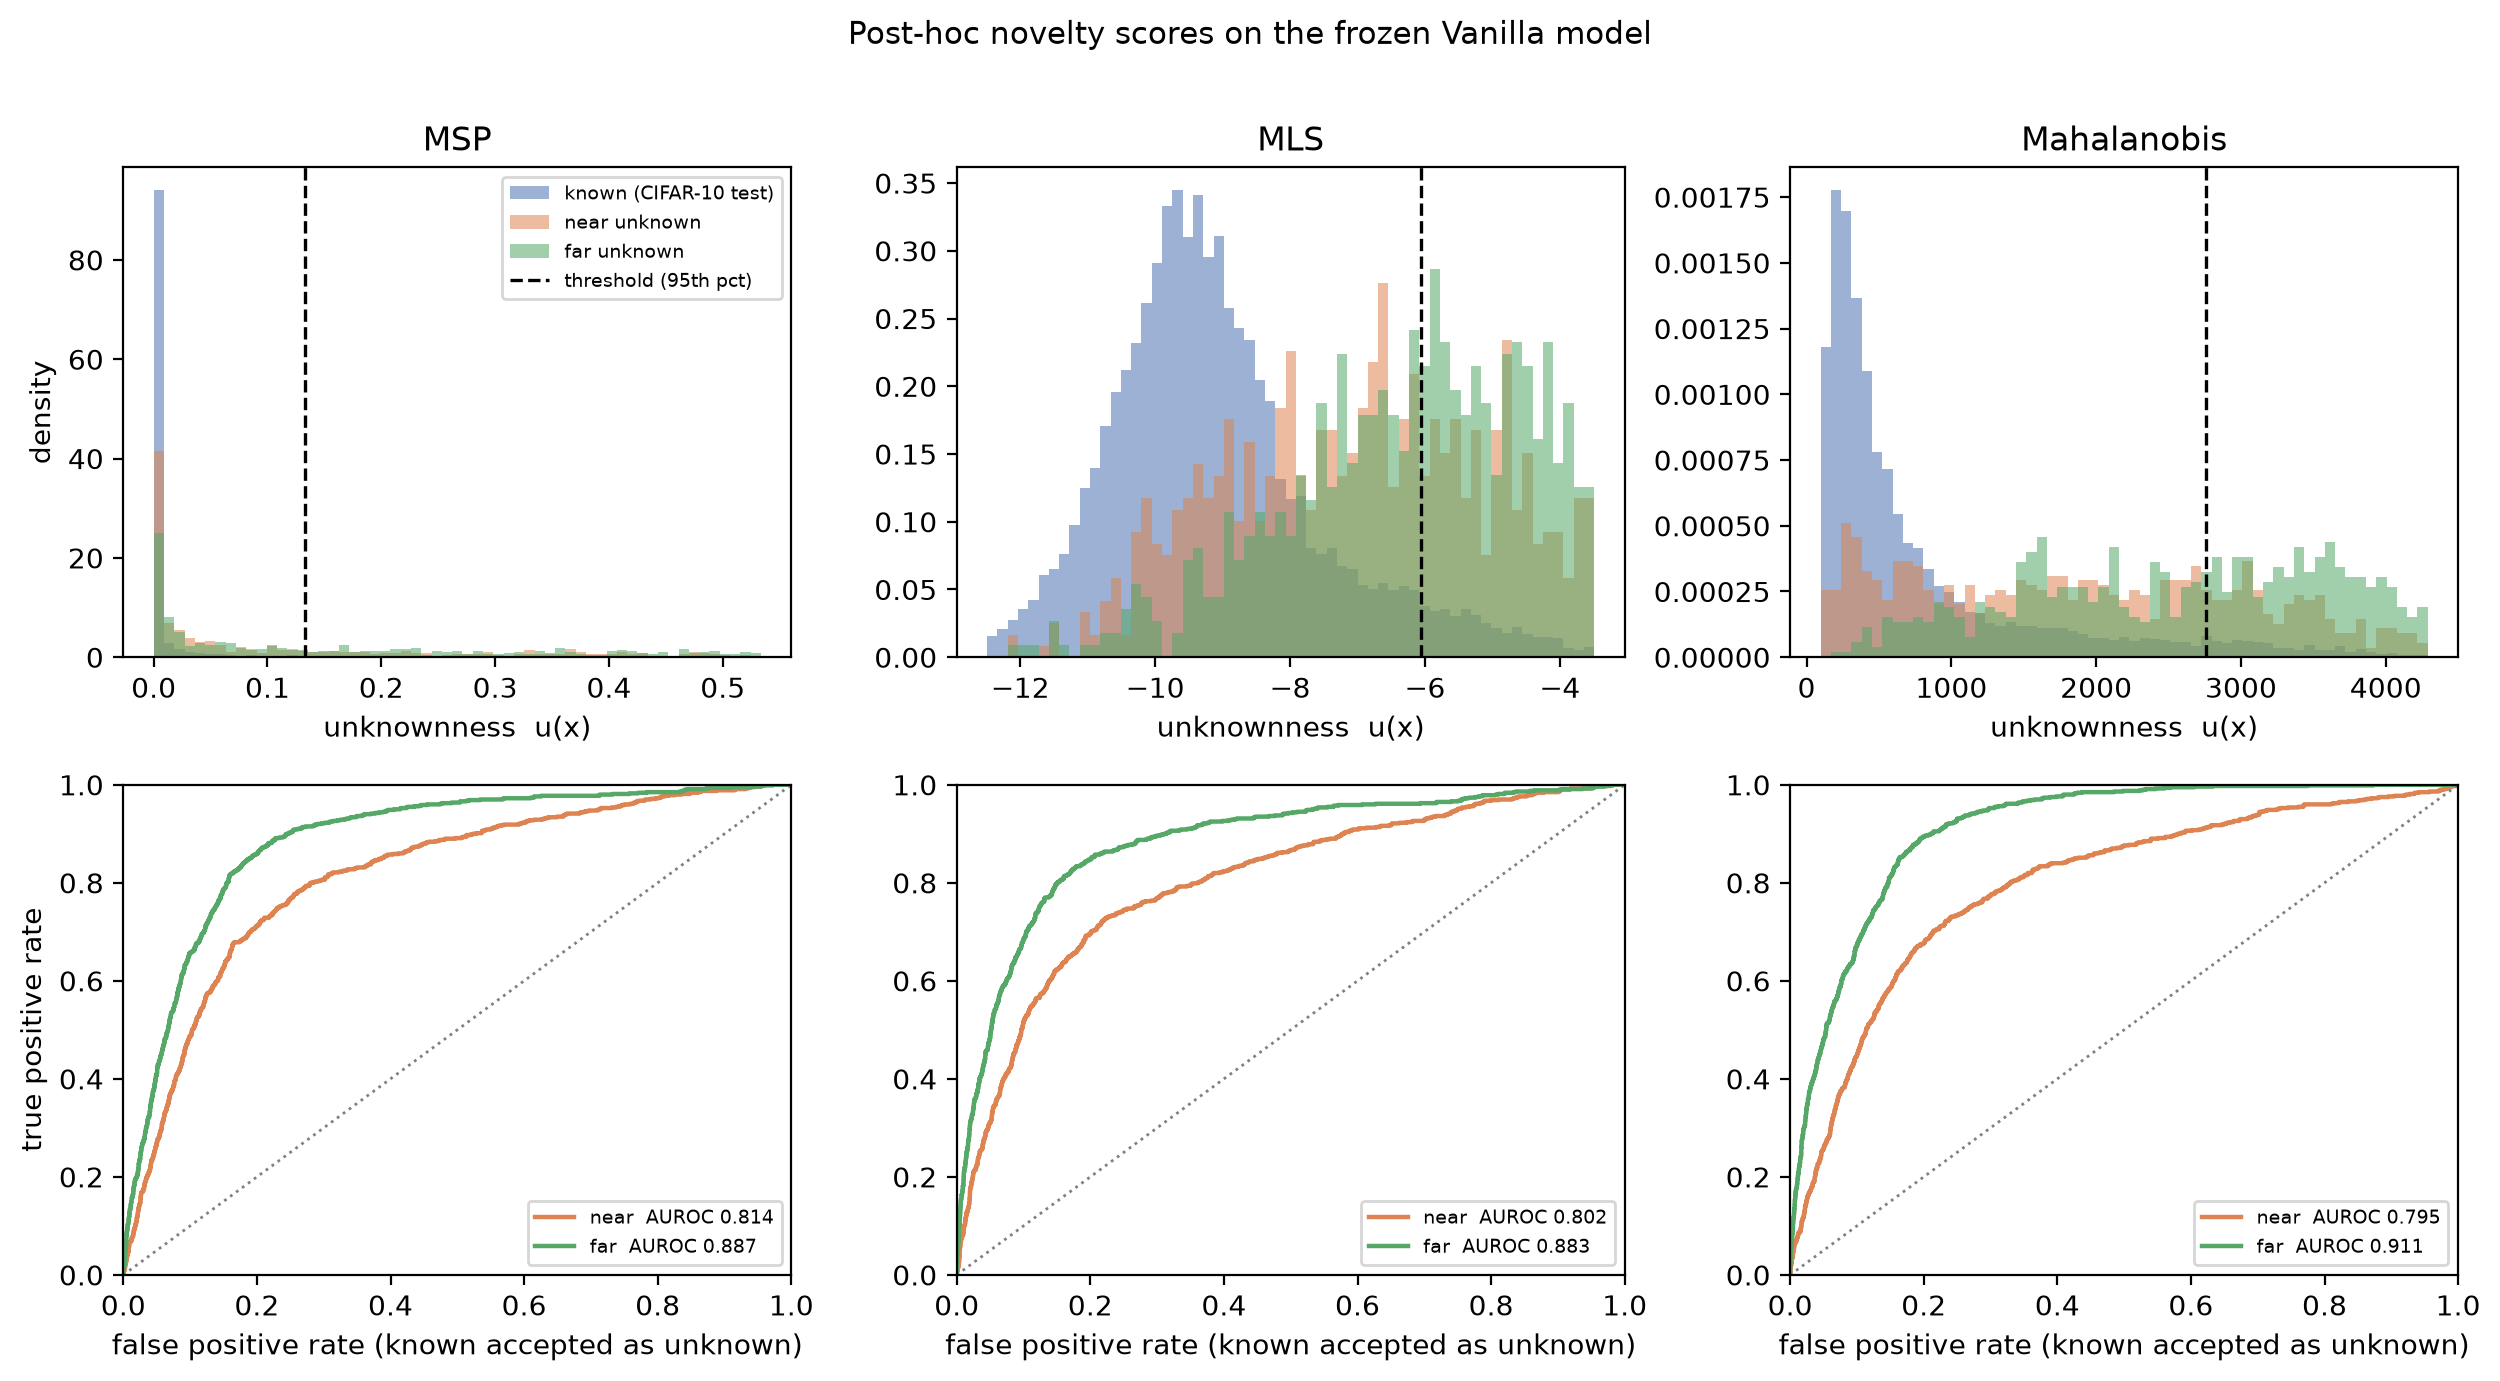
\includegraphics[width=\textwidth]{figures/task4/fig1_osr_scores.png}
  \caption{MSP, MLS and Mahalanobis on Vanilla. Top: unknownness distributions with the threshold (dashed). Bottom: ROC curves for known against near and far unknowns.}
  \label{fig:task4_scores}
\end{figure}

MSP measures relative softmax confidence, where the dominant probability is considered as known-like, and the probabilities spread across classes are unknowns. Given as
MSP unknownness is:
\[ u_{\mathrm{MSP}}(x) = 1-\max_kp_k(x). \]
As compared to MSP, MLS measures the largest absolute logit. The maximum logit represents the strongest raw response of the classifier among the known classes. Given as:

\(u_{\mathrm{MLS}}(x) = -\max_kz_k(x).\)

Here, the negative sign makes the largest value the smallest, representing strength of unknownness: the smaller the \(u_{\mathrm{MLS}}(x)\) the more known the class is.
Where MSP and MLS uses the max single value to compute the unknownness, Energy uses all the classifier logits to compute unknownness, given as:

\[ u_{\mathrm{Energy}}(x) = -\log \sum_{k=1}^{K}e^{z_k(x)}. \]
For CIFAR-10:
\[ K=10. \]
The expression:
\[ \log\sum_ke^{z_k} \]
is called logsumexp.
For large known-class logits, it produces a large total known-class response, which, through the negative, becomes smaller; the small energy means more known.
Mahalanobis measures distance from the nearest known-class feature cluster by calculating a shared diagonal covariance from the training features
For each class:
\[ D_c(x) = (f(x)-\mu_c)^T \Sigma^{-1} (f(x)-\mu_c). \]
Because the covariance is diagonal, this becomes:
\[ D_c(x) = \sum_{j=1}^{512} \frac{ (f_j(x)-\mu_{c,j})^2 }{ \sigma_j^2+\epsilon }. \]
And Mahalanobis novelty score is given as:

\(u_{\mathrm{Mah}}(x) = \min_cD_c(x).\)
I.e., if the feature f(x) is close to at least one known class cluster, the score will be small; otherwise, large.

Novelty scores for all four methods show that classifying far unknowns as unknown was much easier than near unknowns; MLS and energy methods produced almost identical results \(0.802/0.883\) and \(0.802/0.883\) near/far AUROC. This indicates that the largest logit dominated. MSP was most effective for near unknowns, with the highest AUROC of  \(0.814\), which indicates that the relative probability has marginally more information for semantically similar unknowns.

Mahalanobis produced the best far AUROC (\(0.911\)) and the best overall AUROC (\(0.853\)) as well. It shows that for semantically far classes, the feature distance was particularly informative. However, on the contrary, it depicted the weakest near rejection because the near unknowns lie closer to the known clusters, as in the case of wolves and buses, which can lie close to dog or vehicle feature clusters.

Therefore, MSP softmax confidence was most useful for ranking near unknowns, feature distance was strongest for far unknowns, and using all logits through Energy added little beyond MLS in this experiment.

\FloatBarrier
\subsection{Did GCSC Improve Closed-Set and Open-Set Performance?}

\begin{table}[h]
  \caption{Vanilla, GCSC and PROSER with MLS, plus PROSER's placeholder score. CSA uses the ten known-class logits; rejection as in Table~\ref{tab:task4_posthoc}.}
  \label{tab:task4_models}
  \centering
  \small
  \setlength{\tabcolsep}{3.5pt}
  \begin{tabular}{lcccccccc}
    \toprule
    & & \multicolumn{3}{c}{\textbf{AUROC}} & & \multicolumn{3}{c}{\textbf{Rejection (\%)}} \\
    \cmidrule(lr){3-5} \cmidrule(lr){7-9}
    \textbf{Model (score)} & CSA (\%) & Near & Far & All & Known (\%) & Near & Far & All \\
    \midrule
    Vanilla (MLS)            & 94.54 & 0.802 & 0.883 & 0.842 & 94.22 & 34.75 & 54.13 & 44.44 \\
    GCSC (MLS)               & \textbf{95.12} & \textbf{0.826} & \textbf{0.909} & \textbf{0.868} & 94.60 & \textbf{37.13} & \textbf{59.00} & \textbf{48.06} \\
    PROSER (MLS)             & 94.63 & 0.803 & 0.887 & 0.845 & 94.64 & 32.75 & 50.00 & 41.38 \\
    PROSER (placeholder)     & 94.63 & 0.780 & 0.886 & 0.833 & 94.91 & 29.88 & 48.25 & 39.06 \\
    \bottomrule
  \end{tabular}
\end{table}

GCSC shows a slight improvement on closed-set performance, where it gained 0.58 points over the vanilla model, which is about 58 images out of 10,000 test images, not a big number. Since we used only one seed for the dataset, this improvement is not something on which we can assert the claim that GCSC improves the closed-set performance. On open-set, the ordered ranking score AUROC on near and far shows a tiny improvement of 0.024 and 0.027, respectively.

While the AUROC gains were roughly the same for both near and far unknowns, at the rejection threshold for near and far unknowns model reports a gain of 2.38 points on near unknown rejections and 4.88 points on far unknown rejections. This suggests that the augmentation might have encouraged a kind of representation that is less dependent on superficial fluctuations in appearances and thus improved known-class recognition and detection of unknowns. However, the augmentation still does not fully resolve the semantic overlap between classes like bus and truck or wolf and dog, and near-semantic novelty remains the harder problem.

\FloatBarrier
\subsection{Did PROSER Improve Rejection, and What Was the CSA Trade-off?}

The PROSER method via MLS reported an AUROC of 0.845, a 0.003 increase over Vanilla (0.842); however, it's still below GCSC (0.868) by 0.023. It reports near and far rejection rates as \(32.75\%\) and \(50.00\%\) respectively, on the lower side compared to both Vanilla \(34.75\%/54.13\%\) and GCSC \(37.13\%/59.00\%\). The closed-set accuracy of \(94.63\%\) is roughly same as of Vanilla (\(94.54\%\)) and GCSC (\(95.12\%\)).

PROSER's own placeholder scores were also weaker, especially on near unknowns compared to MLS, with an AUROC of 0.780 on near and 0.886 on far, and rejection rates of \(29.88\%\) and \(48.25\%\), respectively. The PROSER was fine-tuned for 50 epochs; however, the highest validation accuracy was achieved very early at the 4th epoch, which may explain why the placeholders were weaker, as at that moment the placeholders' loss was still relatively high; thus, the dummy classifiers had not yet learned stronger class boundaries. Later training did reduce the placeholders' loss; however, it destabilized the validation accuracy, which dropped it as low as 53.12\% at epoch 13 and ended at 93.40\% at epoch 50, below the 95.20\% best.

The models' reported results were not strong enough to clearly support the claim that the classifier and the data placeholders tightened the decision boundaries usefully. The interpolation between the known classes appears insufficient to represent the actual near and far unknown distributions. The model reported several confident failures, such as bus/truck and fox/cat, suggesting that the near unknown lies close to a single known class rather than between two knowns. On the other hand, the failures, such as the keyboard/bird and chair/airplane, show that far unknowns may also occupy directions not represented by interpolating known-class features.


\clearpage
\appendix
\section{Additional Figures}

\begin{figure}[h]
  \centering
  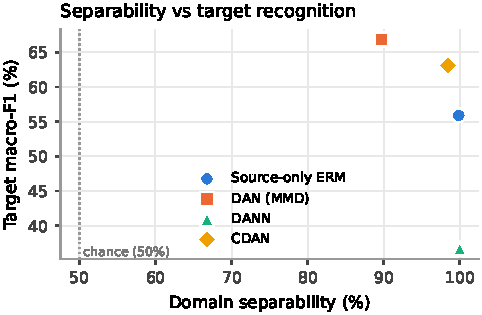
\includegraphics[width=0.5\textwidth]{figures/task2/fig3_separability.pdf}
  \caption{Target macro-F1 against source-vs-target separability for the four Task 2 methods; the dotted line marks chance (50\%).}
  \label{fig:task2_separability}
\end{figure}

\begin{figure}[h]
  \centering
  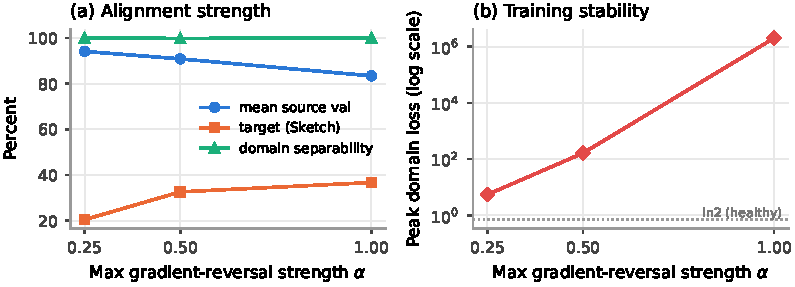
\includegraphics[width=0.72\textwidth]{figures/task2/fig5_alignment_study.pdf}
  \caption{DANN with $\alpha_{\max}\in\{0.25,0.5,1\}$: source macro-F1, target macro-F1 and separability, with the ERM target macro-F1 for reference.}
  \label{fig:task2_alignment_study}
\end{figure}

\begin{figure}[h]
  \centering
  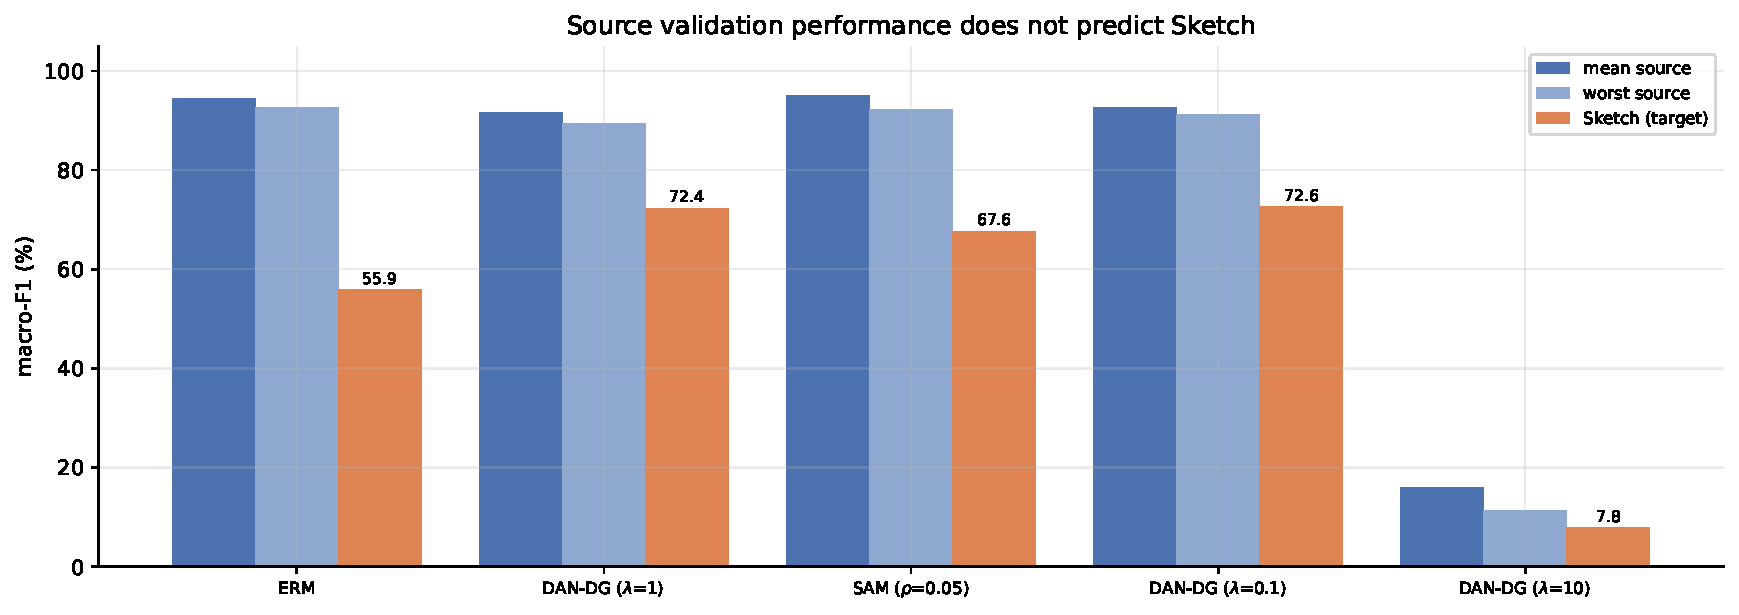
\includegraphics[width=\textwidth]{figures/task3/fig2_method_comparison.pdf}
  \caption{Mean-source, worst-source and Sketch macro-F1 for all Task 3 models.}
  \label{fig:task3_method_comparison}
\end{figure}

\begin{figure}[h]
  \centering
  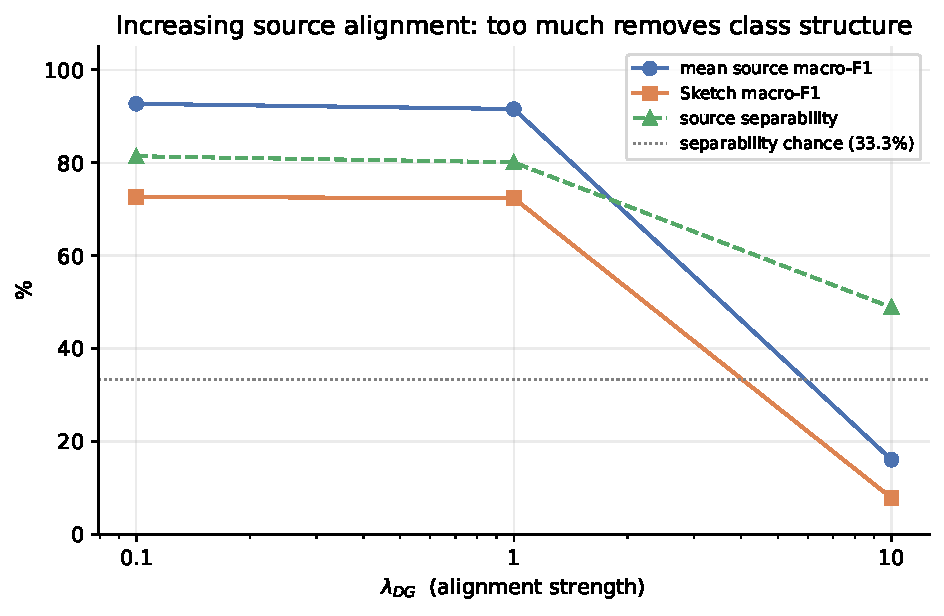
\includegraphics[width=0.62\textwidth]{figures/task3/fig3_alignment_study.pdf}\\[4pt]
  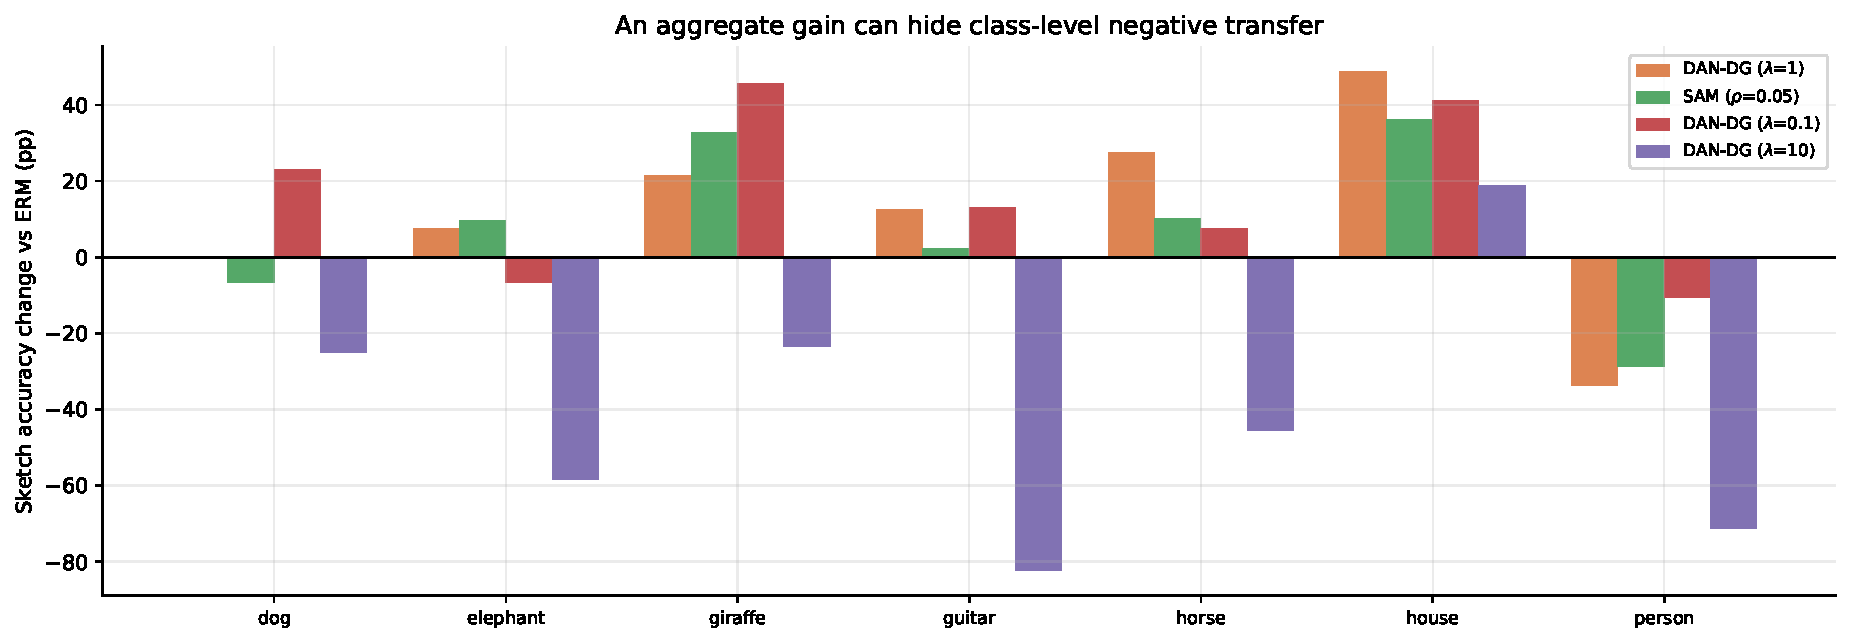
\includegraphics[width=\textwidth]{figures/task3/fig4_per_class.pdf}
  \caption{Top: $\lambda_{\mathrm{DG}}$ study (mean source macro-F1, Sketch macro-F1, source separability; dotted line is chance). Bottom: per-class Sketch accuracy change against ERM.}
  \label{fig:task3_alignment}
\end{figure}

\begin{figure}[h]
  \centering
  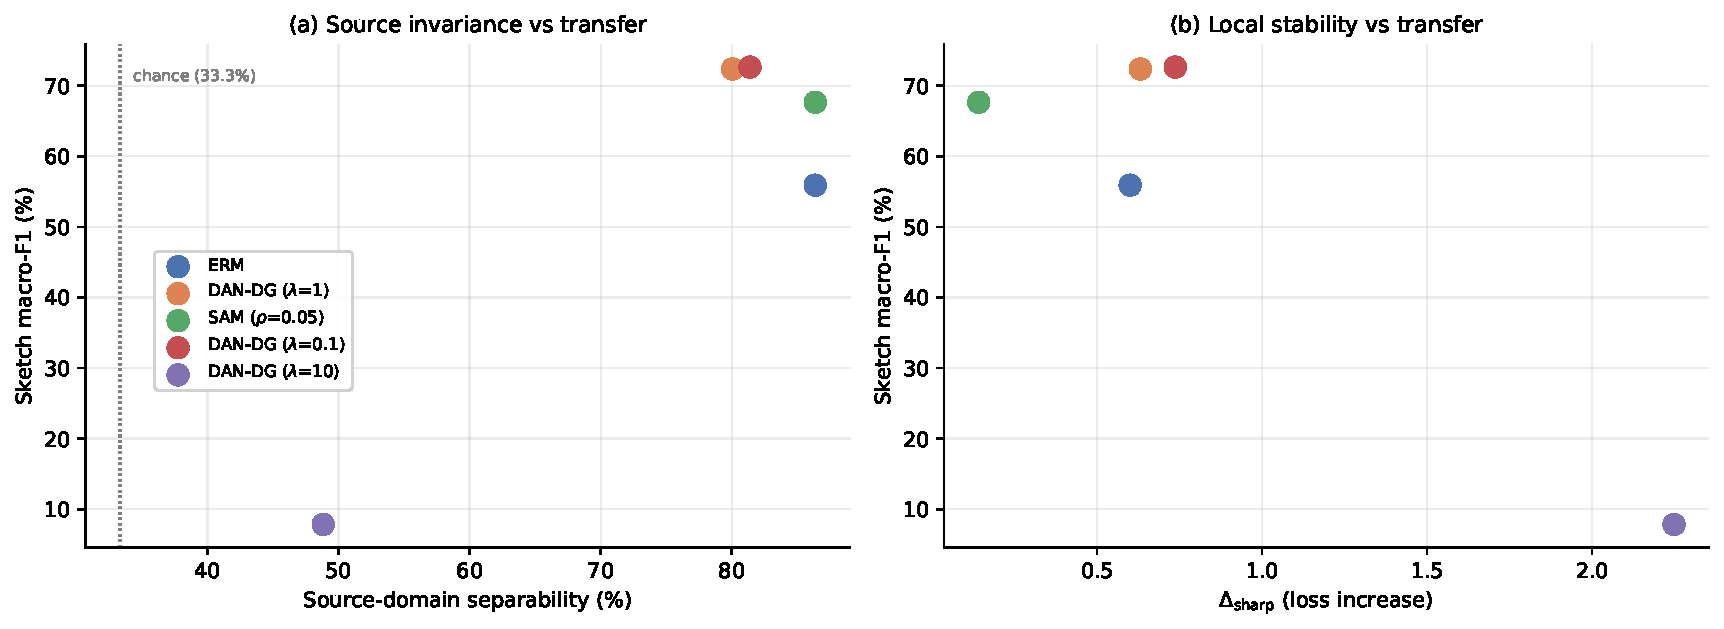
\includegraphics[width=\textwidth]{figures/task3/fig5_diagnostics.pdf}
  \caption{Sketch macro-F1 against (a) source-domain separability and (b) the sharpness proxy $\Delta_{\mathrm{sharp}}$.}
  \label{fig:task3_diagnostics}
\end{figure}

\begin{figure}[h]
  \centering
  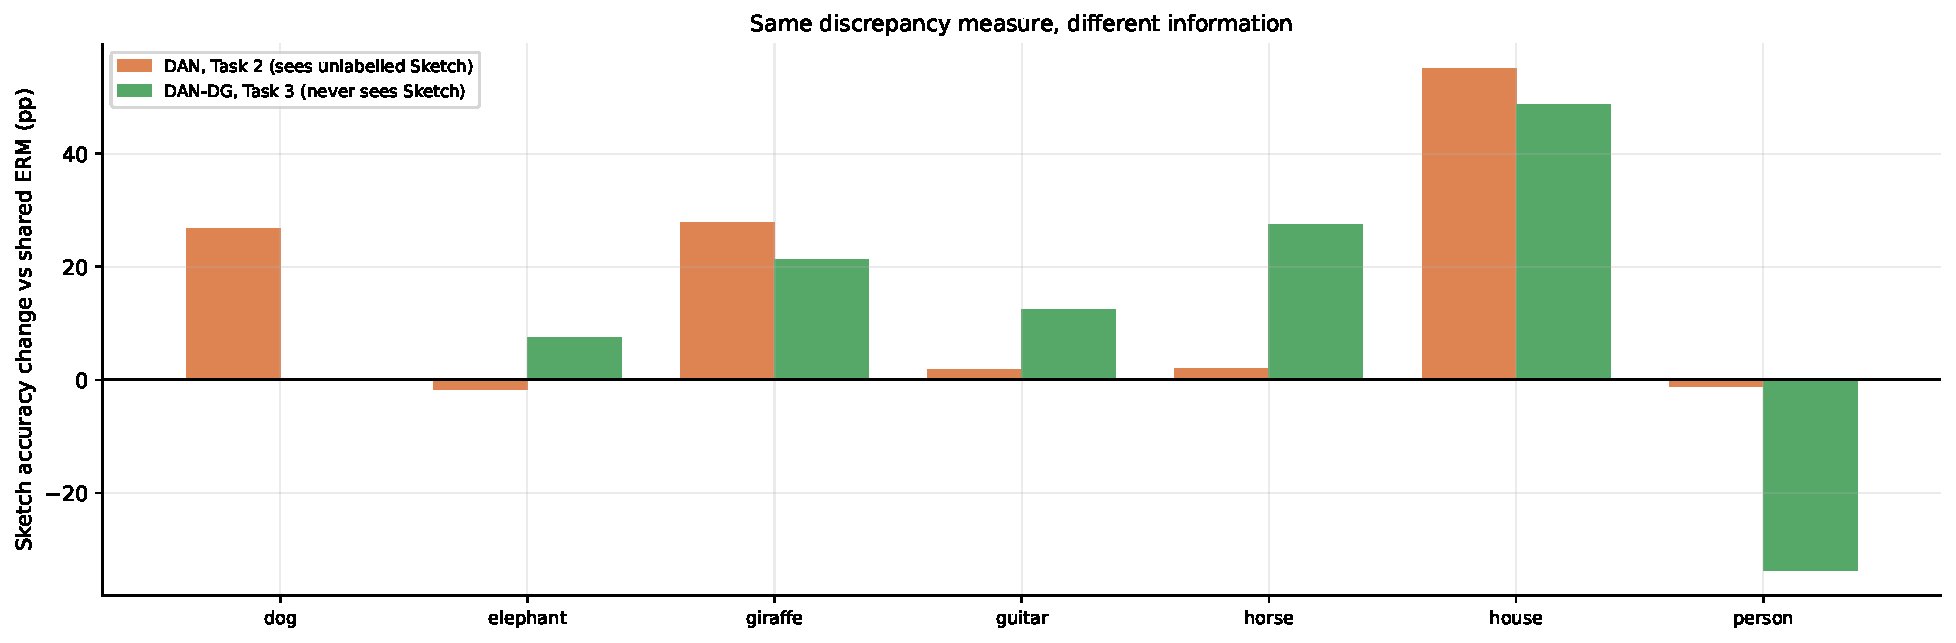
\includegraphics[width=\textwidth]{figures/task3/fig7_per_class_vs_task2.pdf}
  \caption{Per-class Sketch accuracy change against the shared ERM for DAN (Task 2) and DAN-DG (Task 3).}
  \label{fig:task3_vs_task2}
\end{figure}

\begin{figure}[h]
  \centering
  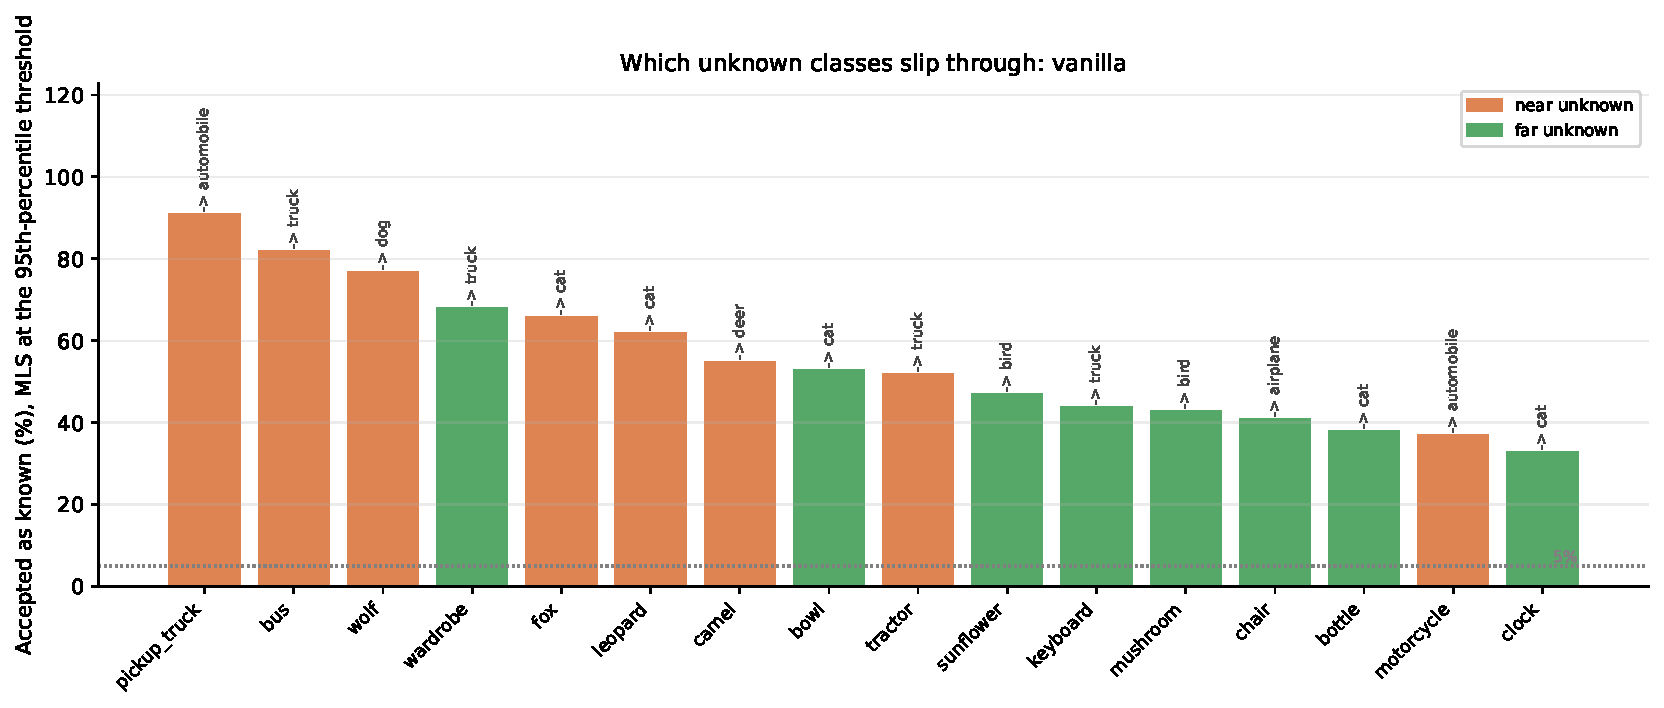
\includegraphics[width=\textwidth]{figures/task4/fig2_unknown_classes.pdf}
  \caption{Share of each unknown class accepted by Vanilla under MLS, annotated with the absorbing CIFAR-10 class (100 images per class).}
  \label{fig:task4_unknown_classes}
\end{figure}


\end{document}
